\thispagestyle{empty}

\noindent
\begin{tabular}{@{}p{11cm}r@{}}
\textbf{ಡಾ. ಡಿ.ಟಿ. ಬಸವರಾಜ್​,}\newline ಕನ್ನಡ ಪ್ರಾಧ್ಯಾಪಕರು,\newline ಕರ್ನಾಟಕ ರಾಜ್ಯ ಮುಕ್ತ ವಿಶ್ವವಿದ್ಯಾನಿಲಯ,\newline ಮುಕ್ತ ಗಂಗೋತ್ರಿ, ಮೈಸೂರು. & \raisebox{-2cm}{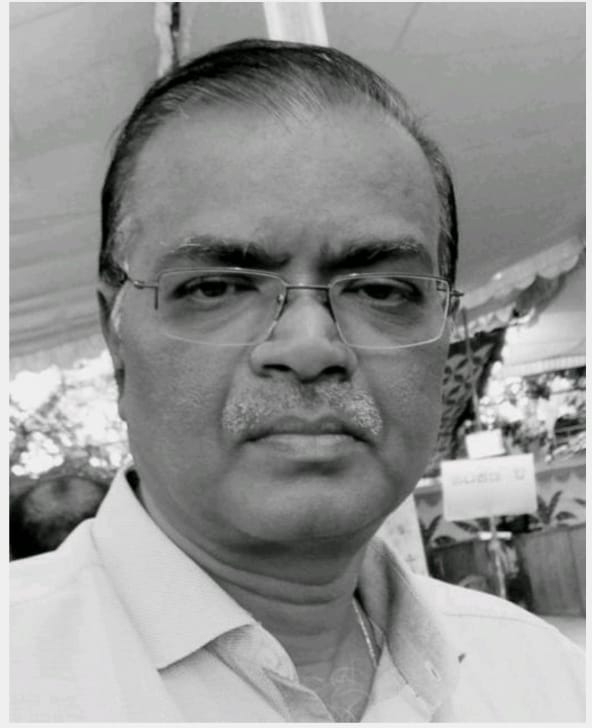
\includegraphics[scale=1.15]{"images/dtb.jpg"}}
\end{tabular}

\noindent
\rule{\textwidth}{1pt}

\bigskip

ಮಂಡ್ಯ ಜಿಲ್ಲೆಯ, ಕೃಷ್ಣರಾಜಪೇಟೆ ತಾಲ್ಲೂಕಿನ, ಸಂತೇಬಾಚಹಳ್ಳಿ ಗ್ರಾಮದ ಎಸ್​. ನಂಜುಂಡಸ್ವಾಮಿಯವರು ನನ್ನ ವಿದ್ಯಾರ್ಥಿ. ಅಧ್ಯಯನದ ಬಗೆಗಿನ ಅವರ ಆಸಕ್ತಿ ಮತ್ತು ಪ್ರೀತಿಯು ಅವರನ್ನು ನನ್ನ ‘ಪ್ರೀತಿಯ ವಿದ್ಯಾರ್ಥಿ’ಯಾಗಿಸಿತು.  ಅವರು ನನ್ನ ಮಾರ್ಗದರ್ಶನದಲ್ಲಿ ಮಂಡ್ಯ ಜಿಲ್ಲೆಯ ಶಾಸನಗಳನ್ನು ಕುರಿತು ಸಂಶೋಧನೆ ನಡೆಸಿ ‘ಮಂಡ್ಯ ಜಿಲ್ಲೆಯ ಶಾಸನಗಳು-ಒಂದು ಅಧ್ಯಯನ’ ಎಂಬ ಬೃಹತ್​ ಪ್ರಬಂಧವನ್ನು ರಚಿಸಿ ೨೦೧೩ರಲ್ಲಿ ಪಿಎಚ್​.ಡಿ. ಪದವಿಯನ್ನು ಪಡೆದಿದ್ದಾರೆ.  ಶಾಸನಗಳ ಅಧ್ಯಯನವು ಒಂದು ವಿರಳ ಅಧ್ಯಯನ ಕ್ಷೇತ್ರ. ಹೆಚ್ಚಿನ ಪರಿಶ್ರಮವನ್ನು ಇದು ನಿರೀಕ್ಷಿಸುತ್ತದೆ.  ಅಧ್ಯಯನ ಧೀರತೆ ಇರುವವರು ಮಾತ್ರ ಈ ಕ್ಷೇತ್ರವನ್ನು ಆಯ್ಕೆ ಮಾಡಿಕೊಳ್ಳುತ್ತಾರೆ. ಈ ಧೀರಗುಣವನ್ನು ನಾನು ಎಸ್​. ನಂಜುಂಡಸ್ವಾಮಿಯವರ ಅಧ್ಯಯನ ಕಾರ್ಯದಲ್ಲಿ ಕಂಡಿದ್ದೇನೆ. ಸಂಶೋಧನೆ ನಡೆಸುವ ಕಾರ್ಯದಲ್ಲಿ ಅವರು ಹೊಂದಿದ್ದ ಪ್ರೀತಿ, ತೋರುತ್ತಿದ್ದ ಶ್ರದ್ಧೆ, ಪಡುತ್ತಿದ್ದ\break ಶ್ರಮಗಳು ಗಮನಾರ್ಹ. ವ್ಯಾಪಕವಾದ ಕ್ಷೇತ್ರಕಾರ್ಯ, ಮಹತ್ವದ ದತ್ತಾಂಶಗಳ ಸಂಗ್ರಹ, ವಿಸ್ತೃತವೂ, ಆಳವೂ ಆದ ತರ್ಕ\-ಬದ್ಧವೂ ಆದ ವಿಶ್ಲೇಷಣೆ ಮತ್ತು ಅಚ್ಚುಕಟ್ಟಾದ ಬರವಣಿಗೆಗಳಿಂದ ಅವರ ಸಂಶೋಧನಾ ಪ್ರಬಂಧ ಮಹತ್ವದ ಕೃತಿಯಾಗಿ ಮೂಡಿ ಬಂದಿದೆ.  ನಂಜುಂಡಸ್ವಾಮಿಯವರ ವಿದ್ವದ್ಸಾಧನೆ ಬಗ್ಗೆ ನನಗೆ ಹೆಮ್ಮೆ ಇದೆ. ಮುಂದುವರಿದು ಅವರ ವಿನಯ, ವ್ಯವಧಾನ ಮತ್ತು ಸಜ್ಜನಿಕೆ ಬಗ್ಗೆ ನನಗೆ ಗೌರವ ಇದೆ.

ಪಿಎಚ್​.ಡಿ. ಅಧ್ಯಯನದ ನಂತರವೂ ಕೂಡಾ ಈ ನಿಟ್ಟಿನಲ್ಲಿ ಹೆಚ್ಚಿನ ಸಂಶೋಧನೆ, ಅಧ್ಯಯನ ಹಾಗೂ ಕ್ಷೇತ್ರ\-ಕಾರ್ಯವನ್ನು  ಮುಂದುವರಿಸಿ,  ಅನೇಕ ಹೊಸ ವಿಷಯಗಳನ್ನು ಸೇರಿಸಿ, ಕೆಲವು ವಿಷಯಗಳನ್ನು ಮಾರ್ಪಾಡು ಮಾಡಿ, \textbf{“ಮಂಡ್ಯ ಜಿಲ್ಲೆಯ ಶಾಸನ ಮತ್ತು ಸಂಸ್ಕೃತಿ” ಎಂಬ ಮಹತ್ವಪೂರ್ಣವಾದ ಬೃಹತ್​ ಸಂಶೋಧನಾ ಕೃತಿಯನ್ನು ರಚಿಸಿದ್ದಾರೆ}. ಈ ಕೃತಿಯ ಒಂದೊಂದು ಅಧ್ಯಾಯವೂ ಒಂದೊಂದು ಸ್ವತಂತ್ರ ಸಂಶೋಧನಾ ಪ್ರಬಂಧಕ್ಕೆ ಆಕರ ಸಾಮಗ್ರಿಯಾಗ ಬಹುದಾಗಿದೆ.  ಮಂಡ್ಯ ಜಿಲ್ಲೆಯ ಪ್ರಾಚೀನ ಇತಿಹಾಸ ಮತ್ತು ಸಂಸ್ಕೃತಿಯ ಬಗ್ಗೆ ಸಮಗ್ರವಾದ ಖಚಿತವಾದ ಮಾಹಿತಿಯನ್ನು ನೀಡುತ್ತದೆ. ಇಂತಹ ಕೃತಿಗಳು ಪ್ರತಿಯೊಂದು ಜಿಲ್ಲೆಯ ಬಗ್ಗೆಯೂ ರಚನೆಯಾದಲ್ಲಿ, ನಾಡಿನ ಇತಿಹಾಸ ಮತ್ತು ಸಂಸ್ಕೃತಿಯ  ತಿಳಿವಳಿಕೆಗೆ ಮತ್ತು ಪುನರ್​ ರಚನೆಗೆ ಸಹಾಯಕವಾಗುತ್ತದೆಂದು ನನ್ನ ಅನಿಸಿಕೆ. 

ಇಂತಹ ಮಹತ್ವದ ಕೃತಿಯನ್ನು ರಚಿಸಿದ ನನ್ನ ವಿದ್ಯಾರ್ಥಿ ಡಾ. ಎಸ್​. ನಂಜುಂಡಸ್ವಾಮಿಯವರಿಗೆ ಅಭಿನಂದನೆಗಳು.  ಈ ಕೃತಿಯನ್ನು ಮಂಡ್ಯ ಜಿಲ್ಲೆಯ ಹಾಗೂ ನಾಡಿನ ಜನತೆ ಆದರದಿಂದ ಬರಮಾಡಿಕೊಳ್ಳುತ್ತಾರೆಂಬ ವಿಶ್ವಾಸ ನನಗಿದೆ. 


\medskip
\bigskip

\noindent
\hfill \textbf{ಡಾ. ಡಿ.ಟಿ. ಬಸವರಾಜ್}

